\documentclass[11pt]{article}
\usepackage[utf8]{inputenc}
\usepackage[T1]{fontenc}
\usepackage{amsmath}
\usepackage{multicol}
\usepackage{geometry}
\usepackage{tikz}
\usetikzlibrary{shapes.geometric, arrows, calc, 3d, shadows}
\usepackage{enumitem}
\usepackage{xcolor}
\usepackage{titlesec}
\usepackage{tcolorbox}

% Configurações
\geometry{a4paper, left=1cm, right=1cm, top=0.5cm, bottom=1.2cm}
\setlength{\columnseprule}{0.4pt}
\definecolor{titleblue}{RGB}{0,80,150}
\definecolor{explanationbg}{RGB}{240,248,255}

% Estilos TikZ
\tikzset{
    solid/.style={draw=black, fill=titleblue!10, thick},
    hollow/.style={draw=titleblue, thick, dashed},
    dimensao/.style={font=\scriptsize, sloped}
}

\title{\textcolor{titleblue}{Atividade de Volume}}
\author{Professor: Jefferson}
\date{}

\begin{document}

\maketitle
\begin{multicols}{2}

\begin{enumerate}[leftmargin=*, itemsep=0.8cm]

%% QUESTÃO 1
\item \textbf{Cubo}: Calcule o volume de um cubo com aresta de 5 cm.

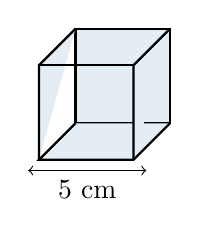
\begin{tikzpicture}[scale=0.6, baseline=-0.5ex]
    \draw[solid] (0,0,0) -- (2,0,0) -- (2,2,0) -- (0,2,0) -- cycle;
    \draw[solid] (0,0,0) -- (0,0,2) -- (2,0,2) -- (2,0,0);
    \draw[solid] (2,0,2) -- (2,2,2) -- (2,2,0);
    \draw[solid] (0,2,0) -- (0,2,2) -- (0,0,2);
    \draw[solid] (0,2,2) -- (2,2,2);
    \draw[<->] (-1,-1.0,0) -- node[below] {5 cm} (1.5,-1.0,0);
\end{tikzpicture}

%% QUESTÃO 2
\item \textbf{Paralelepípedo}: Determine o volume desta caixa retangular em litros (1L $=$ 1000 cm³).  

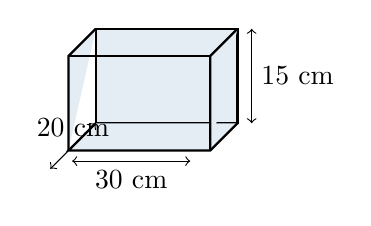
\begin{tikzpicture}[scale=0.6, baseline=-0.5ex]
    \draw[solid] (0,0,0) -- (3,0,0) -- (3,2,0) -- (0,2,0) -- cycle;
    \draw[solid] (0,0,0) -- (0,0,1.5) -- (3,0,1.5) -- (3,0,0);
    \draw[solid] (3,0,1.5) -- (3,2,1.5) -- (3,2,0);
    \draw[solid] (0,2,0) -- (0,2,1.5) -- (0,0,1.5);
    \draw[solid] (0,2,1.5) -- (3,2,1.5);
    \draw[<->] (3.3,0,0) -- node[right] {15 cm} (3.3,2,0);
    \draw[<->] (-0.5,-0.8,0) -- node[below] {30 cm} (2,-0.8,0);
    \draw[<->] (0,0,2.5) -- node[above] {20 cm} (0,0,0);
\end{tikzpicture}

%% QUESTÃO 3
\item \textbf{Cilindro}: Qual o volume deste cilindro? (Use $\pi = 3,14$)

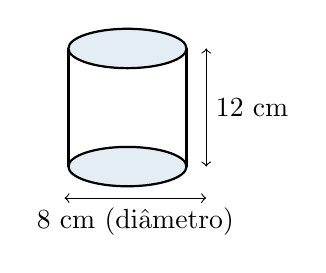
\begin{tikzpicture}[scale=0.5, baseline=-0.5ex]
    \draw[solid] (0,0) ellipse (1.5 and 0.5);
    \draw[solid] (-1.5,0) -- (-1.5,3);
    \draw[solid] (1.5,0) -- (1.5,3);
    \draw[solid] (0,3) ellipse (1.5 and 0.5);
    \draw[dashed] (-1.5,0) arc (180:360:1.5 and 0.5);
    \draw[<->] (-1.6,-0.8) -- node[below] {8 cm (diâmetro)} (2.0,-0.8);
    \draw[<->] (2,0) -- node[right] {12 cm} (2,3);
\end{tikzpicture}

%% QUESTÃO 4
\item \textbf{Esfera}: Determine o raio $r$ desta esfera.  
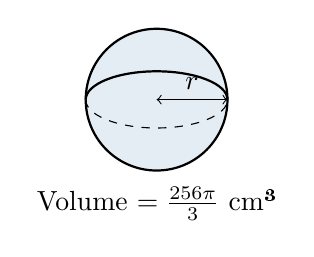
\begin{tikzpicture}[scale=0.6, baseline=-0.5ex]
    \draw[solid] (0,0) circle (1.5);
    \draw[dashed] (-1.5,0) arc (180:360:1.5 and 0.6);
    \draw[solid] (1.5,0) arc (0:180:1.5 and 0.6);
    \draw[<->] (0,0) -- node[above] {$r$} (1.5,0);
    \node at (0,-2.2) {Volume $ = \frac{256\pi}{3}$ cm³};
\end{tikzpicture}

%% QUESTÃO 5
\item \textbf{Cone}: Calcule o volume deste cone.  

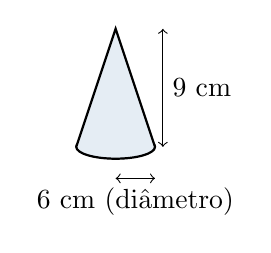
\begin{tikzpicture}[scale=0.5, baseline=-0.5ex]
    \draw[solid] (0,0) ellipse (1 and 0.3);
    \draw[solid] (-1,0) -- (0,3) -- (1,0);
    \draw[dashed] (-1,0) arc (180:360:1 and 0.3);
    \draw[<->] (1.2,0) -- node[right] {9 cm} (1.2,3);
    \draw[<->] (0,-0.8) -- node[below] {6 cm (diâmetro)} (1,-0.8);
\end{tikzpicture}

%% QUESTÃO 6
\item \textbf{Pirâmide Quadrada}: Qual o volume desta pirâmide?  

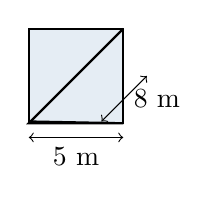
\begin{tikzpicture}[scale=0.6, baseline=-0.5ex]
    \draw[solid] (0,0) -- (2,0) -- (2,2) -- (0,2) -- cycle;
    \draw[solid] (1,1,2.5) -- (0,0) -- (2,0) -- cycle;
    \draw[solid] (1,1,2.5) -- (2,2);
    \draw[dashed] (1,1,2.5) -- (1,1,0);
    \draw[<->] (0,-0.3) -- node[below] {5 m} (2,-0.3);
    \draw[<->] (2.5,1) -- node[right] {8 m} (2.5,1,2.5);
\end{tikzpicture}


%% QUESTÃO 7
\item \textbf{Prisma Triangular}: Calcule o volume deste prisma. 

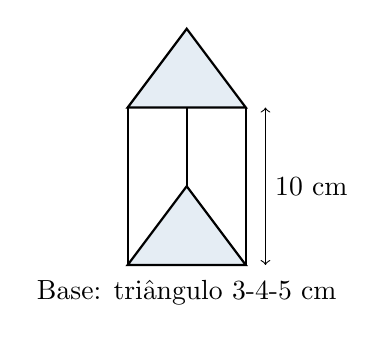
\begin{tikzpicture}[scale=0.5, baseline=-0.5ex]
    \draw[solid] (0,0) -- (3,0) -- (1.5,2) -- cycle;
    \draw[solid] (0,0) -- (0,4);
    \draw[solid] (3,0) -- (3,4);
    \draw[solid] (1.5,2) -- (1.5,6);
    \draw[solid] (0,4) -- (3,4) -- (1.5,6) -- cycle;
    \node at (1.5,-0.7) {Base: triângulo 3-4-5 cm};
    \draw[<->] (3.5,0) -- node[right] {10 cm} (3.5,4);
\end{tikzpicture}


%% QUESTÃO 8
\item \textbf{Tronco de Cone}: Determine o volume deste tronco de cone.  

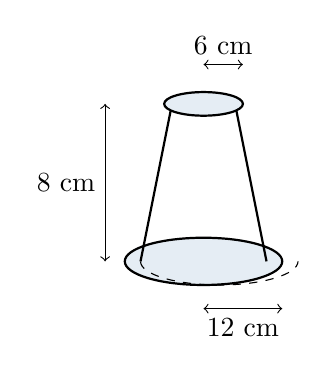
\begin{tikzpicture}[scale=0.5, baseline=-0.5ex]
    \draw[solid] (0,0) ellipse (2 and 0.6);
    \draw[solid] (-1.6,0) -- (-0.8,4);
    \draw[solid] (1.6,0) -- (0.8,4);
    \draw[solid] (0,4) ellipse (1 and 0.3);
    \draw[dashed] (-1.6,0) arc (180:360:2 and 0.6);
    \draw[<->] (0,-1.2) -- node[below] {12 cm} (2,-1.2);
    \draw[<->] (0,5) -- node[above] {6 cm} (1,5);
    \draw[<->] (-2.5,0) -- node[left] {8 cm} (-2.5,4);
\end{tikzpicture}


%% QUESTÃO 9
\item \textbf{Octaedro}: Calcule o volume deste octaedro regular.  

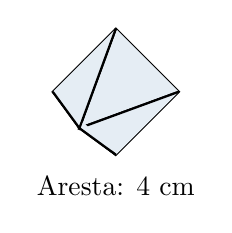
\begin{tikzpicture}[scale=0.4, baseline=-0.5ex]
    \draw[solid] (0,2) -- (2,0) -- (0,-2) -- (-2,0) -- cycle;
    \draw[solid] (0,2) -- (0,0,3) -- (2,0);
    \draw[solid] (2,0) -- (0,0,3) -- (0,-2);
    \draw[solid] (0,-2) -- (0,0,3) -- (-2,0);
    \draw[solid] (-2,0) -- (0,0,3) -- (0,2);
    \node at (0,-3) {Aresta: 4 cm};
\end{tikzpicture}


%% QUESTÃO 10
\item \textbf{Cilindro Oco}: Qual o volume de metal deste cano?
  
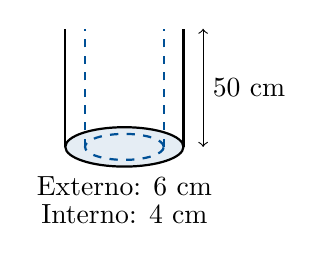
\begin{tikzpicture}[scale=0.5, baseline=-0.5ex]
    \draw[solid] (0,0) ellipse (1.5 and 0.5);
    \draw[hollow] (0,0) ellipse (1 and 0.33);
    \draw[solid] (-1.5,0) -- (-1.5,3);
    \draw[solid] (1.5,0) -- (1.5,3);
    \draw[hollow] (-1,0) -- (-1,3);
    \draw[hollow] (1,0) -- (1,3);
    \node at (0,-1) {Externo: 6 cm};
    \node at (0,-1.7) {Interno: 4 cm};
    \draw[<->] (2,0) -- node[right] {50 cm} (2,3);
\end{tikzpicture}

%% QUESTÃO 11
\item \textbf{Tetraedro}:Calcule o volume deste tetraedro regular.
 
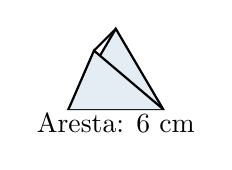
\begin{tikzpicture}[scale=0.6, baseline=-0.5ex]
    \draw[solid] (0,0) -- (2,0) -- (1,1.7) -- cycle;
    \draw[solid] (0,0) -- (1,1.7,1.2) -- (2,0);
    \draw[solid] (1,1.7) -- (1,1.7,1.2);
    \draw[dashed] (0,0) -- (1,1.7,1.2) -- (1,1.7);
    \node at (1,-0.3) {Aresta: 6 cm};
\end{tikzpicture}

%% QUESTÃO 12
\item \textbf{Prisma Hexagonal Regular}  
Um prisma hexagonal regular possui aresta da base medindo 2 cm e altura de 15 cm, conforme ilustrado abaixo.

\begin{tikzpicture}[scale=0.6, baseline=-0.5ex]
    % Base inferior
    \foreach \i in {0,...,5} {
        \draw[solid] (60*\i:1.5) -- (60*\i:1.5,3);
        \draw[solid, fill=titleblue!10] (60*\i:1.5) -- (60*\i+60:1.5) -- (60*\i+60:1.5,3) -- (60*\i:1.5,3) -- cycle;
    }
    % Arestas da base superior
    \draw[solid] (0:1.5,3) -- (60:1.5,3) -- (120:1.5,3) -- (180:1.5,3) -- (240:1.5,3) -- (300:1.5,3) -- cycle;
    % Destaque para uma face lateral
    \draw[solid, fill=titleblue!5] (0:1.5) -- (60:1.5) -- (60:1.5,3) -- (0:1.5,3) -- cycle;
    % Dimensões
    \draw[<->] (0,-2.5) -- node[below] {2 cm} (60:1.5,-2.0);
    \draw[<->] (2.2,0) -- node[right] {15 cm} (2.2,3);
    % Eixo central
    \draw[dashed] (0,0) -- (0,3);
\end{tikzpicture}

Determine:
\begin{enumerate}[label=(\alph*)]
    \item A área da base hexagonal
    \item O volume do prisma
\end{enumerate}

%% QUESTÃO 13
\item \textbf{Anel Esférico}: Qual o volume da parte azul?
  
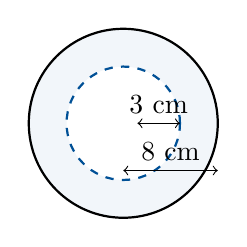
\begin{tikzpicture}[scale=0.6, baseline=-0.5ex]
    \draw[solid, fill=titleblue!5] (0,0) circle (2);
    \draw[hollow, fill=white] (0,0) circle (1.2);
    \draw[<->] (0,-1) -- node[above] {8 cm} (2,-1);
    \draw[<->] (0.3,0) -- node[above] {3 cm} (1.2,0);
\end{tikzpicture}

%% QUESTÃO 14
\item \textbf{Cilindro Inscrito}:Qual o volume do cilindro inscrito no cubo?
 
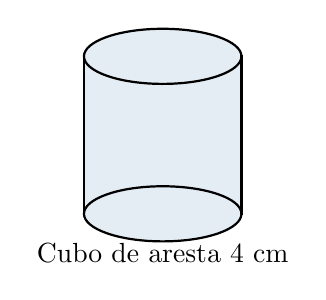
\begin{tikzpicture}[scale=0.5, baseline=-0.5ex]
    \draw[solid] (0,0) -- (4,0) -- (4,4) -- (0,4) -- cycle;
    \draw[solid] (2,0) ellipse (2 and 0.7);
    \draw[solid] (2,4) ellipse (2 and 0.7);
    \draw[solid] (0,0) -- (0,4);
    \draw[solid] (4,0) -- (4,4);
    \node at (2,-1) {Cubo de aresta 4 cm};
\end{tikzpicture}

%% QUESTÃO 15
\item \textbf{Cones Gêmeos}  
Dois cones idênticos compartilham a mesma base circular. Sabendo que o raio da base é 4 cm e a altura de cada cone é 6 cm, calcule o volume total da figura.

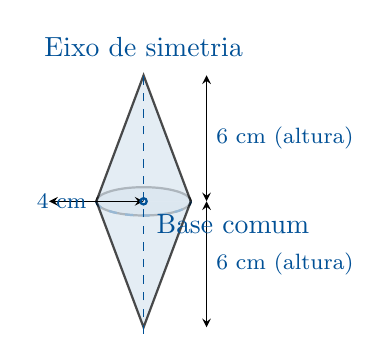
\begin{tikzpicture}[scale=0.4, baseline=-0.5ex]
    % Estilos
    \tikzset{
        cone/.style={solid, fill=titleblue!15, opacity=0.7},
        dimensao/.style={font=\footnotesize, text=titleblue}
    }
    
    % Base compartilhada (preenchida)
    \draw[cone] (0,0) ellipse (1.5 and 0.45);
    \draw[hollow] (-1.5,0) arc (180:360:1.5 and 0.45);
    
    % Cone superior (transparente)
    \draw[cone] (-1.5,0) -- (0,4) -- (1.5,0);
    
    % Cone inferior (transparente)
    \draw[cone] (-1.5,0) -- (0,-4) -- (1.5,0);
    
    % Dimensões
    \draw[<->, >=stealth] (0,0) -- node[left, dimensao] {4 cm} (-3.0,0); % Raio
    \draw[<->, >=stealth] (2,0) -- node[right, dimensao] {6 cm (altura)} (2,4); % Altura cone superior
    \draw[<->, >=stealth] (2,0) -- node[right, dimensao] {6 cm (altura)} (2,-4); % Altura cone inferior
    
    % Linha de simetria tracejada
    \draw[dashed, titleblue] (0,-4.2) -- (0,4.2);
    \node[titleblue, above] at (0,4.3) {Eixo de simetria};
    
    % Destaque da base compartilhada
    \draw[titleblue, thick] (0,0) circle (0.1);
    \node[titleblue, below right] at (0.1,-0.1) {Base comum};
\end{tikzpicture}


%% QUESTÃO 16
\item \textbf{Pirâmide Cortada}: Calcule o volume deste tronco de pirâmide.
 
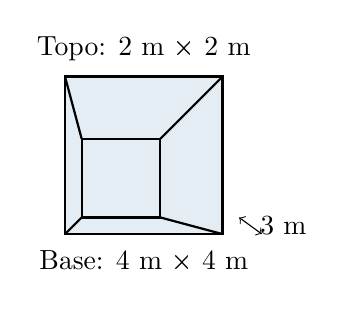
\begin{tikzpicture}[scale=0.5, baseline=-0.5ex]
    \draw[solid] (0,0) -- (4,0) -- (4,4) -- (0,4) -- cycle;
    \draw[solid] (1,1,1.5) -- (3,1,1.5) -- (3,3,1.5) -- (1,3,1.5) -- cycle;
    \draw[solid] (0,0) -- (1,1,1.5);
    \draw[solid] (4,0) -- (3,1,1.5);
    \draw[solid] (4,4) -- (3,3,1.5);
    \draw[solid] (0,4) -- (1,3,1.5);
    \node at (2,-0.7) {Base: 4 m × 4 m};
    \node at (2,4.7) {Topo: 2 m × 2 m};
    \draw[<->] (5,0) -- node[right] {3 m} (5,1,1.5);
\end{tikzpicture}

%% QUESTÃO 17
\item \textbf{Desafio: Sólido Complexo}: Calcule o volume deste sólido (cilindro + 2 semiesferas).
  

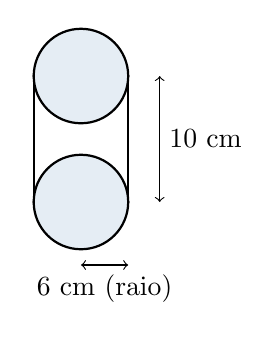
\begin{tikzpicture}[scale=0.4, baseline=-0.5ex]
    % Cilindro central
    \draw[solid] (0,0) ellipse (1.5 and 0.5);
    \draw[solid] (-1.5,0) -- (-1.5,4);
    \draw[solid] (1.5,0) -- (1.5,4);
    \draw[solid] (0,4) ellipse (1.5 and 0.5);
    % Semiesferas
    \draw[solid] (0,0) circle (1.5);
    \draw[solid] (0,4) circle (1.5);
    % Dimensões
    \draw[<->] (2.5,0) -- node[right] {10 cm} (2.5,4);
    \draw[<->] (0,-2) -- node[below] {6 cm (raio)} (1.5,-2);
\end{tikzpicture}

\end{enumerate}
\end{multicols}

\vspace{0.5cm}
\begin{tcolorbox}[colback=titleblue!5, colframe=titleblue, title=\textbf{Fórmulas Úteis: }]
\begin{multicols}{2}
\begin{itemize}
\item Cubo: $V = a^3$
\item Paralelepípedo: $V = abc$
\item Cilindro: $V = \pi r^2 h$
\item Cone: $V = \frac{1}{3}\pi r^2 h$
\item Esfera: $V = \frac{4}{3}\pi r^3$
\item Pirâmide: $V = \frac{1}{3}A_b h$
\item Tronco de cone: $V = \frac{\pi h}{3}(R^2 + Rr + r^2)$
\item Octaedro: $V = \frac{\sqrt{2}}{3}a^3$
\item Prisma: $V = A_b \times h$
\item Semiesfera: $V = \frac{2}{3}\pi r^3$
\end{itemize}
\end{multicols}
\end{tcolorbox}

\end{document}
